\paragraph{\texttt{FeedbackCard}}  \mbox{}\\

This component presents a card for a specific feedback, encompassing the name of the student who authored it, the comment, and the date of publication.
Prior to \texttt{CourseCard}, the first table of is relatively straightforward.


\begin{center}
    \begin{tabularx}{\textwidth}{|X|X|X|X|}
        \hline
        \textbf{Prop} & Type & Required & Description \\
        \hline
        \texttt{feedback} & \texttt{Feedback} & yes & A yoga feedback \\
        \hline
    \end{tabularx}
\end{center}

And more precisely

%\begin{center}
%    \begin{tabularx}{\textwidth}{|X|X|X|}
%        \hline
%        \textbf{Prop.attribute} & Type & Description \\
%        \hline
%        \texttt{feedback.photo} & \texttt{string | null} &  the path of  the yoga feedback's profile photo stored in Supabase\\
%        \hline
%        \texttt{feedback.name} & \texttt{string} & the name of the yoga feedback\\
%        \hline
%        \texttt{feedback.biography} & \texttt{string} & the biography of the feedback\\
%        \hline
%        \texttt{feedback.certificates} & \texttt{string[]} & a list of yoga certifications\\
%        \hline
%    \end{tabularx}
%\end{center}

\begin{figure}[H]
    \centering
    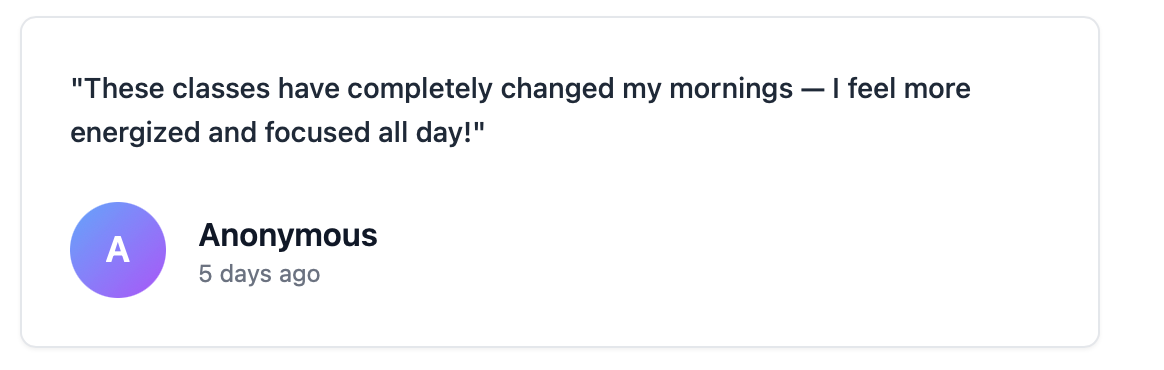
\includegraphics[width=0.4\textwidth]{asset/feedbackCard}
    \caption{\texttt{feedbackCard}}
\end{figure}